\section{Interfacing with Applications}

\ken{
  Each subsection should be up to 2/3 pages plus have images up to 1/2 page.
  (3.5 pages total.)
  The section should start with a layperson overview of what the domain problem is, what scientists are doing to study the problem.
  The section should then explain how visualization fits in to help.
  Explain the technical solution of how VTK-m was integrated into the system and describe the final result.
  The section may repeat for multiple things that were done.
  For example the fusion reactor could first talk about in situ images and then Poincar\'{e} plots.
  The laser wakefields could talk about deliver of in situ images via Ascent and then about the customized particle advection.
  The final section will be a little different in that it will iterate over multiple science domains.
}

\subsection{Tokamak Fusion Reactor}

\assign{Dave}

Fusion energy research is focused on understanding the science needed to develop energy sources based on the controlled fusion of light atomic nuclei. This is done in a device called a tokamak that uses magnetic fields to confine a hot plasma in the shape of a torus.
Significant efforts are currently underway to prepare for ITER, the large experimental reactor under construction in France.
The Whole Device Model Application (WDMApp) is a project in ECP that aims to develop a high-fidelity model of magnetically confined fusion plasma in tokamaks. 
WDMApp is critical in the efforts to plan experiments on ITER and optimize the design of future next-step fusion facilities. These devices will operate in physics regimes not achieved by any current or past experiments, making advanced and predictive numerical simulation the best tool for the task.


%WDMApp is focused on building the main driver and coupling framework for the more complete Whole Device Model (WDM), with the ultimate goal of completing a comprehensive computational suite that includes all the physics components required to simulate a magnetically confined fusion reactor. The main driver for the WDM will be the coupling of two advanced gyrokinetic codes, one in the edge (XGC~\cite{XGC}) and the other in the core (GENE~\cite{GENE} or GEM~\cite{GEM}). XGC is a particle-in-cell (PIC) code optimized for treating the edge plasma. While GENE is a continuum code, GEM is a PIC code optimized for the core plasma. WDMApp takes advantage of the complementary nature of these two applications in the core to build the most advanced and efficient whole-device kinetic transport kernel for the WDM, and also to mitigate risk.


The behavior and evolution of the magnetic field in a tokamak is complex, and its control is critical for performance.
Because of this, analysis tools for understanding the dynamic nature of the magnetic field are critical.
The complexity of the three-dimensional magnetic field lines makes analysis and visualization difficult.
Because the field lines are periodic, this complexity can be reduced by using a \poincare magnetic field-line puncture map~\cite{Sanderson2010}. 
The \poincare map is the intersection of a field line with a lower-dimensional subspace (called the \poincare section).
In our case, the \poincare section is a two-dimensional plane that is perpendicular to the axis of the tokamak.
Given a set of magnetic field lines, the \poincare map, or intersections of magnetic field lines with the plane provides a concise 
representation of the magnetic field that is easier to understand and analyze.

In practice, the \poincare map is generated by creating a large number of field lines and plotting each intersection, or puncture, with the plane.
After a sufficient number of punctures have been collected, patterns in the map characterize the features in the magnetic field.
The field lines are computed by advecting many massless particles through the magnetic field.
The intersections generated from a single particle characterize the features of the magnetic surface at that position.
The particles are advected using a differential equation solver, such as the 4$^{th}$ order Runge-Kutta scheme (RK4).

In practice, proper characterization of the magnetic field requires a large number of intersections (typically between 1000 and 3000) and initial positions (typically tens of thousands).
Because of this, the computation of a \poincare map can be very expensive.
The WDMApp team has a \poincare map code that runs on CPUs and takes several hours for the largest analysis runs. 
%Because of this cost, the generation \poincare maps required careful planning.
The high cost of the analysis was due to two main factors. First, the large numbers of particles and intersections required previously mentioned, and second, the complexity of the magnetic field calculation.  In many applications of particle advection, the vector field is calculated at the nodes of each cell in the mesh. Linear interpolation within the cell is used to evaluate the magnetic field for the particle being advected. Because of the large number of advection steps required for each particle in the \poincare map, small errors can rapidly accumulate. These errors are compounded by the fact that the evaluation of the magnetic field requires a complex set of calculations requiring high-order interpolation of several quantities.

\begin{figure*}[ht]
  \centering
%  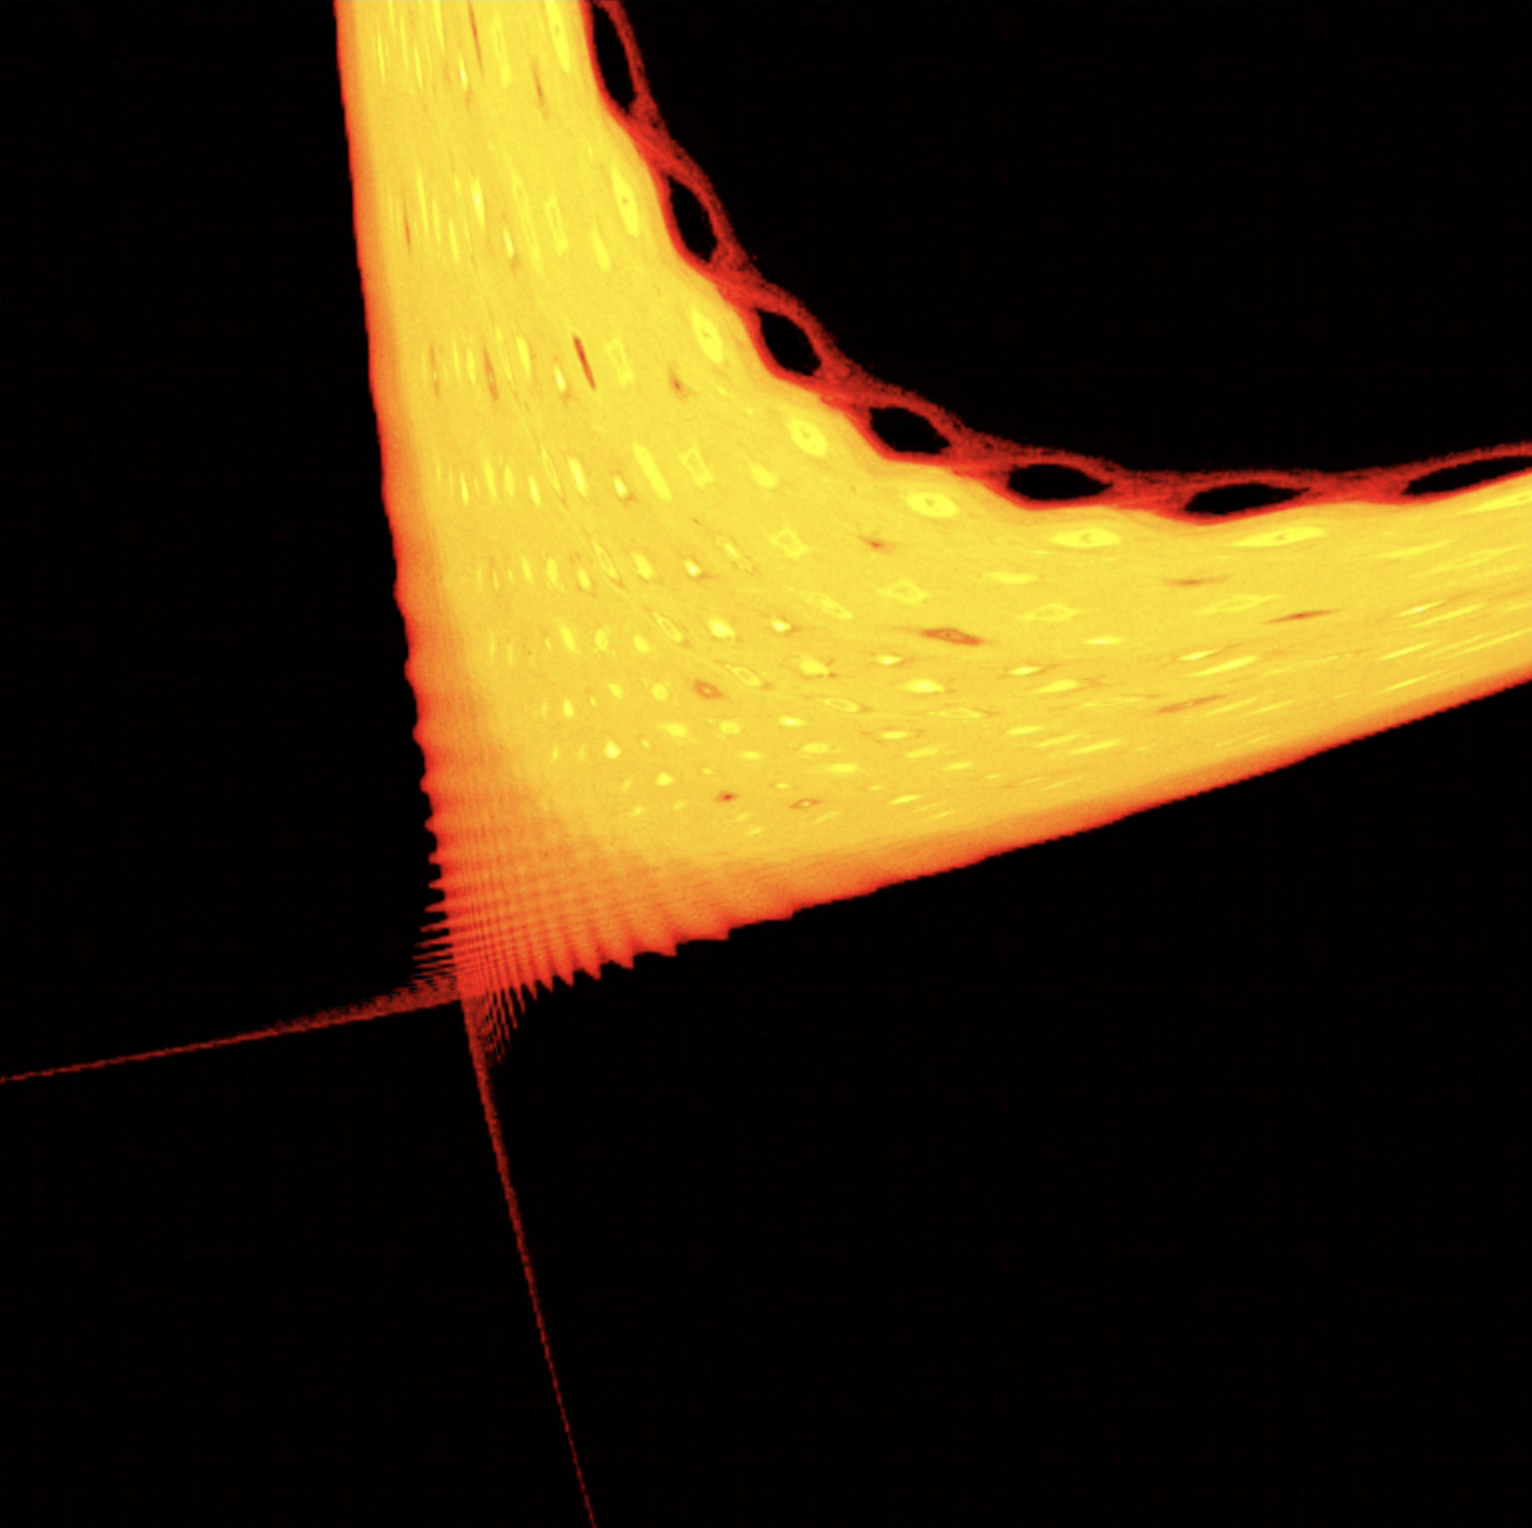
\includegraphics[width=0.49\linewidth]{figures/poincare1}
%  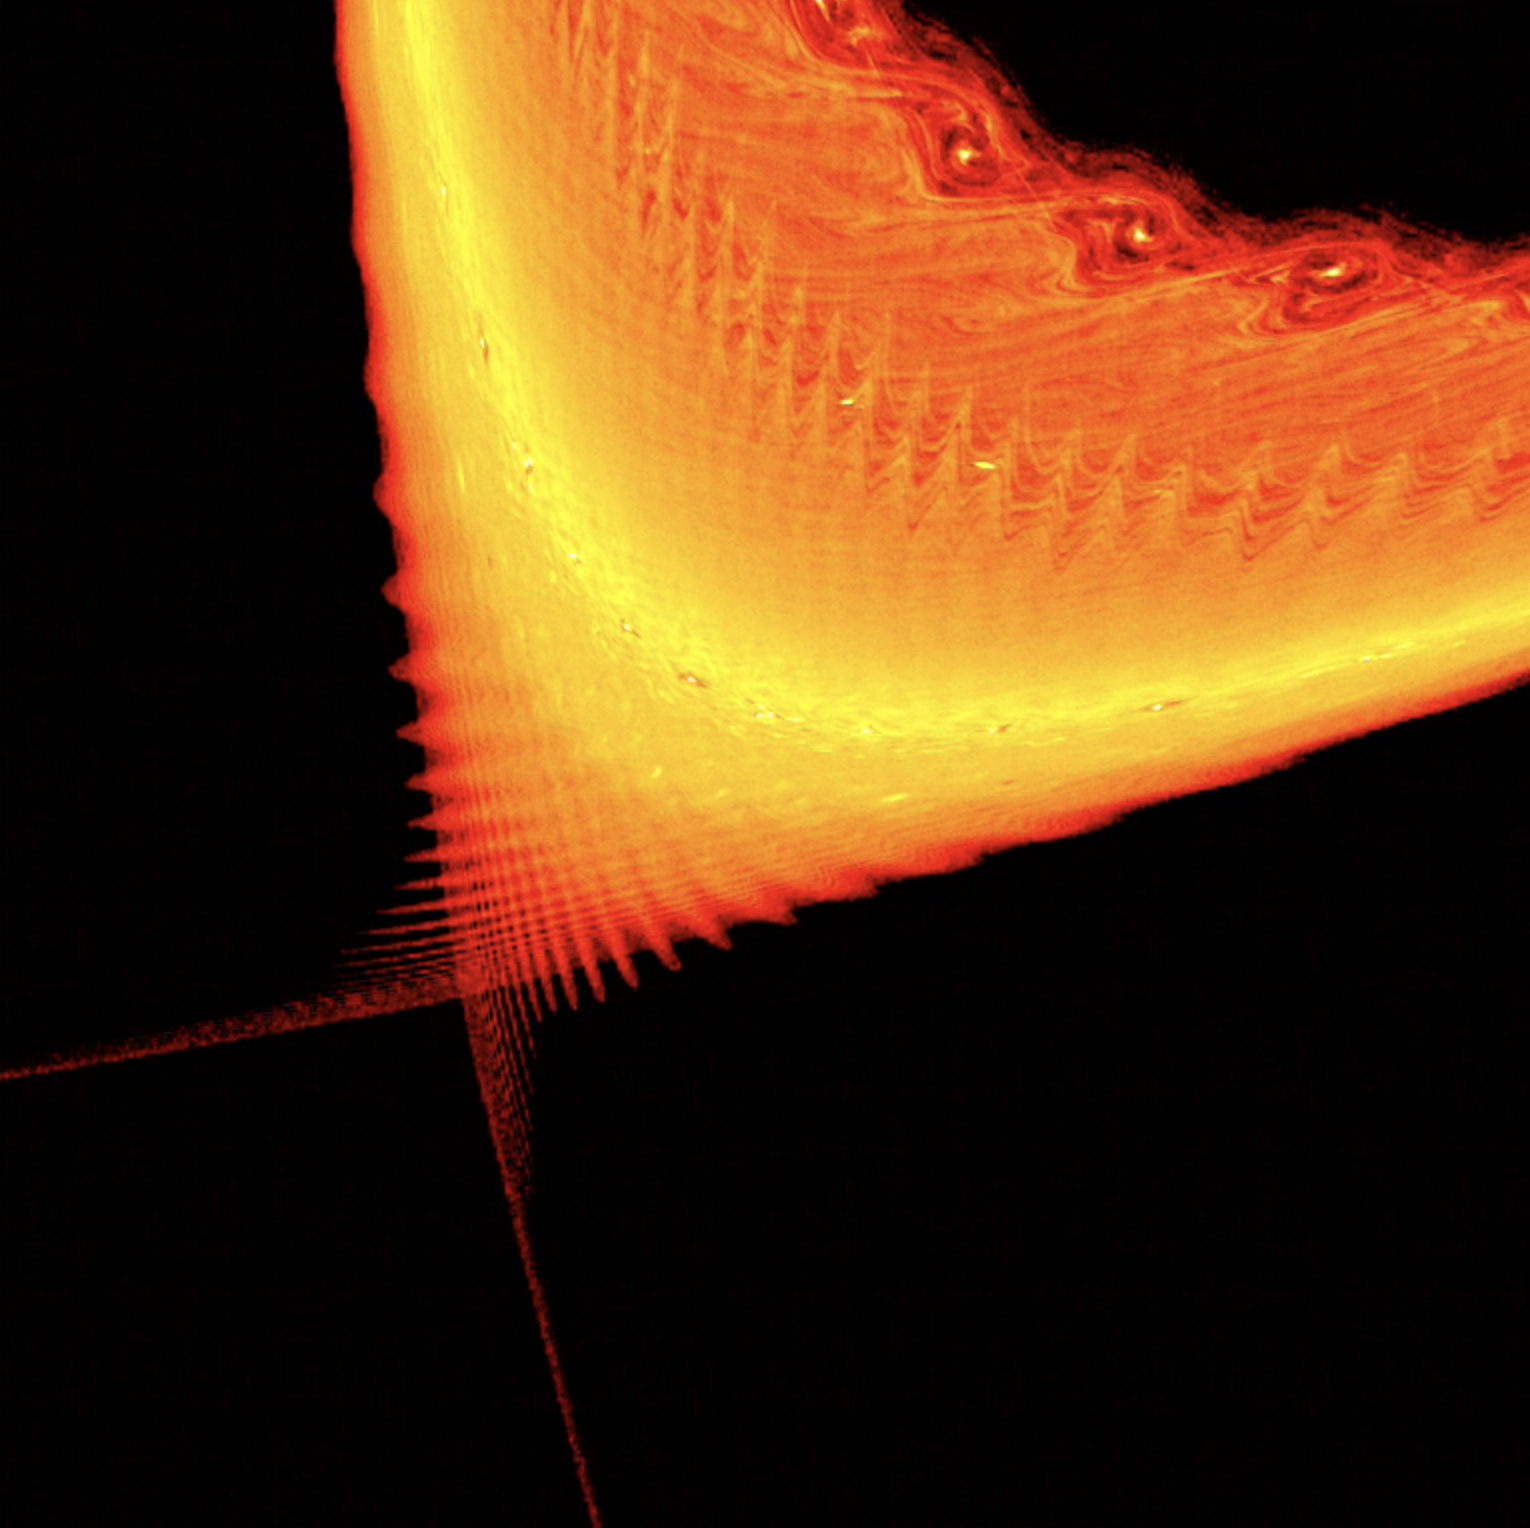
\includegraphics[width=0.49\linewidth]{figures/poincare2}
  \caption{\poincare maps.}
  \label{fig:poincare}
\end{figure*}

Using VTK-m we can significantly accelerate the computation of \poincare maps using the parallelism available on GPUs. Because the trajectory of each particle is completely independent, the task can be parallelized over each particle. Using this approach, a \poincare map can be computed in under $3$ minutes. The wall-clock time for a typical WDMApp simulation step is between $1.5$ and $2$ minutes, which means that \poincare maps can be computed in situ in nearly real-time.
When WDMApp is run, the workflow control system, EFFIS~\cite{Suchyta2022:effis}, allocates an additional 1 to 2 additional nodes for the \poincare map analysis. As a simulation step completes, EFFIS launches a \poincare analysis task on GPUs in the node in a round-robin fashion. This allows asynchronous analysis to be performed on the additional nodes while the simulation is running.
Real-time generation of \poincare maps provides the WDMApp team with unprecedented capability for analysis of magnetic fields in fusion simulations.




\subsection{Laser Wakefield Acceleration}\label{sec:warpx}

\assign{Axel, Abhi}~%
%
%\defcitealias{FedeliHuebl2022}{Fedeli, Huebl et al. (2022)}
%\citepalias{FedeliHuebl2022}
%
WarpX is a particle-in-cell simulation code, which was awarded the 2022 ACM Gordon Bell Prize~\cite{FedeliHuebl2022}.
As part of ECP, WarpX was developed as a new application succeeding its predecessor Warp~\cite{Vay2013}, with the goal to study advanced particle acceleration in laser-driven plasma wakefields, towards future high-energy physics colliders~\cite{Albert2021}.
Beyond that, WarpX is used to describe kinetic physics in particle accelerators, laser-plasmas, fusion devices, inertial confinement fusion and astrophysical plasmas, and is used to model microelectronics~\cite{Yao2022}.

Figure~\ref{fig:warpx_lwfa} is an in situ rendering of a \emph{staged} laser wakefield accelerator in a boosted reference frame~\cite{Vay2011}.
An electron beam (orange-green) is accelerated to the right through multiple stages to high energies.
In the plasma stages (grey), the strong traversal focusing fields are shown in red-blue.

In the staging approach, a particle beam is accelerated subsequently through multiple plasma elements.
In each stage, an ultra-intense laser pulse is exciting a plasma wakefield.
This depletes the laser pulse's energy to generate very strong electric fields in the plasma wake, which can be used to accelerate an injected electron beam.
The acceleration itself can be three to four orders of magnitude more compact than relying on state-of-the-art radio-frequency accelerator elements.
Besides increased beam energy, physicists study how to preserve beam properties essential for transport, focusing (e.g., emittance) and applications (e.g., charge and current).

WarpX features advanced techniques such as GPU-acceleration for three vendors, mesh-refinement capabilities, dynamic load balancing, and unique advanced numerical solvers.
WarpX relies on multi-level parallelization: coarse parallelization relies on block-structured domain-decomposition with MPI using the AMReX library~\cite{Zhang2019} and compute acceleration with CUDA/HIP/SYCL or OpenMP, so that simulations are scalable to the world's largest supercomputers.

If WarpX would only rely on traditional post-processing workflows for visualization of the dynamics of Exascale simulations, the resulting multi-PByte scale output per simulation would severely limit the available snapshots and/or level of detail to visualize.
Addressing this need, its in situ visualization interfaces to Ascent, for which utility routines were implemented in AMReX, which are specialized in WarpX ``diagnostics'' for application-specific descriptions.
WarpX performs data preparation steps for diagnostics in situ and shares the respective AMReX memory buffers with zero-copy APIs through Conduit with Ascent, rendering with VTK-m in the same domain-decomposition and on the same compute device as the simulation itself.

\begin{figure*}[ht]
  \centering
  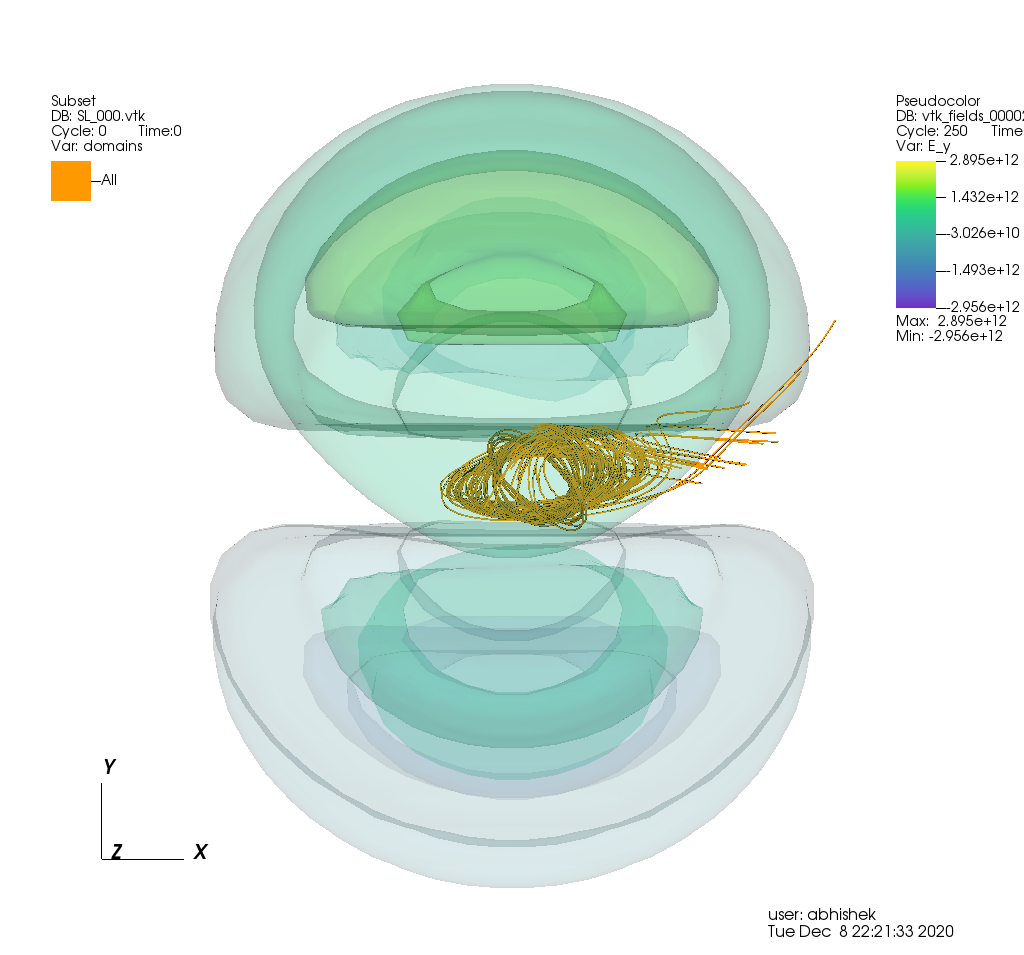
\includegraphics[width=0.49\linewidth]{figures/lwfa_particle_advection_front.png}%
  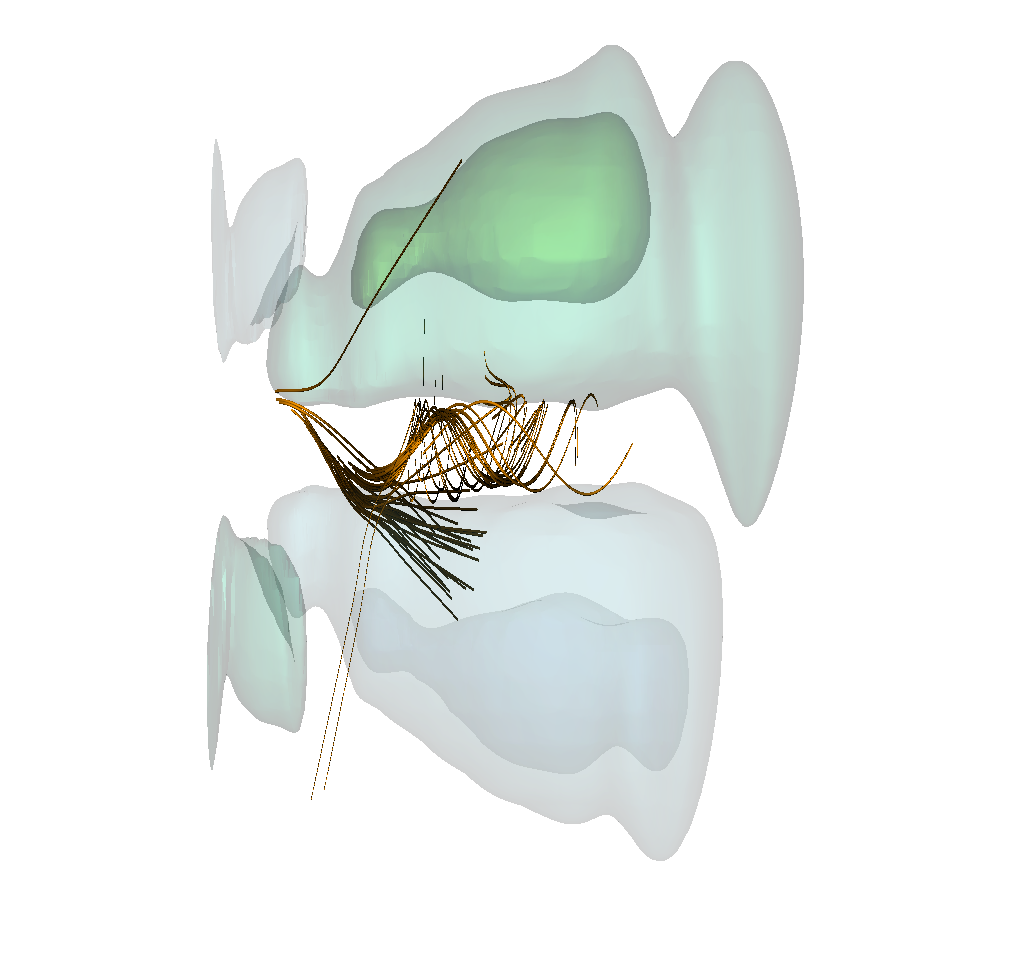
\includegraphics[width=0.49\linewidth]{figures/lwfa_particle_advection_side.png}
  \caption{Side- \& front-view of an laser wakefield with an injected electron bunch.
  Particles are advected from \emph{a single snapshot} of the simulation in VTK-m.}
  \label{fig:lwfa_particle_advection}
\end{figure*}

Realistic visualization of particle trajectories (advection) in a plasma or particle accelerator requires high temporal fidelity in traditional workflows, which can create a high data overhead.
With VTK-m, an opportunity to significantly reduce data input for such workflows was identified, making use of a physics-motivated advection algorithm and the slowly changing nature of fields in a wakefield accelerator.

Plasma particles such as electrons and ions are inert and can be relativistic, which effectively changes their mass as they move.
Traditional advection algorithms only made use of local properties of fields, without a history and inert nature of a streamline.
As in a particle-in-cell algorithm, the realistic track of a charged plasma particle can be integrated following the Lorentz-Force, which interpolates six local field components ($E_{x,y,z}, B_{x,y,z}$) and advances the particles' momentum (inertia) and position with an explicit iteration scheme~\cite{Boris1970}.
The updated momentum is tracked over the path of a streamline to account for the evolving particle.

With this advection algorithm integrated in VTK-m, a snapshot of a simulation can be used to project the particles' physical position forward (and backward) for a meaningful time, under the realistic assumption that fields are quasi-static, i.e., do not change much in time (besides translation along an axis).
Figure~\ref{fig:lwfa_particle_advection} shows such particle trajectories of an off-axis injected electron beam in a wakefield, calculated from a single snapshot, reproducing physical betatron oscillation.

\subsection{Impact Beyond ECP}

\assign{Jay}

%\jay{discuss the applications/use cases outside of ECP}
In addition to the applications mentioned above, VTK-m still serves as the key infrastructure for accelerating data analysis and visualization in various scientific applications through \emph{in situ} approach. This subsection lists several typical examples and illustrates how VTK-m is integrated into \emph{in situ} scientific workflows outside of ECP.


Before being selected as a project in ECP, VTK-m was a core component in Visualization for the Extreme-Scale Scientific Computation Ecosystem (XVis)~\cite{Moreland2019}. 
XVis focused on multiple ways to integrate \emph{in situ} visualization with the simulation, extract key information, and decrease the data size for post-hoc processing.
The ``\emph{in situ} reduction + post hoc'' paradigm is widely adopted in multiple scientific domains, such as probability distribution functions (PDF) extraction of fields in combustion simulation~\cite{Ye2016}, and binning mechanism to reduce the data size of fusion simulation~\cite{Kress2018}. 


Nyx is a cosmological simulation that aims to solve compressible hydrodynamics with N-body treatment of the dark matter. Each simulation run may contain hundreds of time steps with multiple sets of simulation input parameters. The raw data size is usually hundreds of TBs to several PBs, which causes challenges to process data in post-processing. 
VTK-m is used as \emph{in situ} analysis to extract the statistical properties of the down-sampled data to hugely reduce the size of raw data. The associated statistics model can be used to construct the data based on prior knowledge in post-processing with low data reconstruction error~\cite{Wang2019}.

Eddy detection and tracking plays a key role in the ocean simulation field. Understanding the characteristics of eddies can help scientists to explain the regional air-sea interactions.
VTK-m streamline filter can be used as an \emph{in situ} analysis to generate streamline data used for interactive post-hoc analysis~\cite{Han2022}. With the help of VTK-m, the associated eddy analysis workflow can improve the interaction speed, reduce data storage, and meet the
needs of real-time visual analysis interaction.  
